%%%%%%%%%%%%%%%%%%%%%%%%%%%%%%%%%%%%%%%%%%%%%%%%%%%%%%%%%%%%%%%%%%%%%
%% This is a (brief) model paper using the achemso class
%% The document class accepts keyval options, which should include
%% the target journal and optionally the manuscript type. 
%%%%%%%%%%%%%%%%%%%%%%%%%%%%%%%%%%%%%%%%%%%%%%%%%%%%%%%%%%%%%%%%%%%%%
\documentclass[journal=jacsat,manuscript=article]{achemso}

%%%%%%%%%%%%%%%%%%%%%%%%%%%%%%%%%%%%%%%%%%%%%%%%%%%%%%%%%%%%%%%%%%%%%
%% Place any additional packages needed here.  Only include packages
%% which are essential, to avoid problems later. Do NOT use any
%% packages which require e-TeX (for example etoolbox): the e-TeX
%% extensions are not currently available on the ACS conversion
%% servers.
%%%%%%%%%%%%%%%%%%%%%%%%%%%%%%%%%%%%%%%%%%%%%%%%%%%%%%%%%%%%%%%%%%%%%
\usepackage[version=3]{mhchem} % Formula subscripts using \ce{}

%%%%%%%%%%%%%%%%%%%%%%%%%%%%%%%%%%%%%%%%%%%%%%%%%%%%%%%%%%%%%%%%%%%%%
%% If issues arise when submitting your manuscript, you may want to
%% un-comment the next line.  This provides information on the
%% version of every file you have used.
%%%%%%%%%%%%%%%%%%%%%%%%%%%%%%%%%%%%%%%%%%%%%%%%%%%%%%%%%%%%%%%%%%%%%
%%\listfiles

%%%%%%%%%%%%%%%%%%%%%%%%%%%%%%%%%%%%%%%%%%%%%%%%%%%%%%%%%%%%%%%%%%%%%
%% Place any additional macros here.  Please use \newcommand* where
%% possible, and avoid layout-changing macros (which are not used
%% when typesetting).
%%%%%%%%%%%%%%%%%%%%%%%%%%%%%%%%%%%%%%%%%%%%%%%%%%%%%%%%%%%%%%%%%%%%%
\newcommand*\mycommand[1]{\texttt{\emph{#1}}}

%%%%%%%%%%%%%%%%%%%%%%%%%%%%%%%%%%%%%%%%%%%%%%%%%%%%%%%%%%%%%%%%%%%%%
%% Meta-data block
%% ---------------
%% Each author should be given as a separate \author command.
%%
%% Corresponding authors should have an e-mail given after the author
%% name as an \email command. Phone and fax numbers can be given
%% using \phone and \fax, respectively; this information is optional.
%%
%% The affiliation of authors is given after the authors; each
%% \affiliation command applies to all preceding authors not already
%% assigned an affiliation.
%%
%% The affiliation takes an option argument for the short name.  This
%% will typically be something like "University of Somewhere".
%%
%% The \altaffiliation macro should be used for new address, etc.
%% On the other hand, \alsoaffiliation is used on a per author basis
%% when authors are associated with multiple institutions.
%%%%%%%%%%%%%%%%%%%%%%%%%%%%%%%%%%%%%%%%%%%%%%%%%%%%%%%%%%%%%%%%%%%%%
\author{Lyssa M. Freese}
\email{lyssamfreese@gmail.com}
\affiliation[MITeaps]
{Department of Earth, Atmosphere and Planetary Sciences, Massachusetts Institute of Technology}
\author{Guillaume Chossiere}
\author{Sebastian Eastham}
\affiliation{Laboratory for Aviation and the Environment, Department of Aeronautics and Astronautics, Massachusetts Institute of Technology}
\author{Noelle Selin}
\affiliation[MITeaps]{Department of Earth, Atmosphere and Planetary Sciences, Massachusetts Institute of Technology}
\alsoaffiliation[MITidss]
{Institute for Data, Systems and Society, Massachusetts Institute of Technology}

%%%%%%%%%%%%%%%%%%%%%%%%%%%%%%%%%%%%%%%%%%%%%%%%%%%%%%%%%%%%%%%%%%%%%
%% The document title should be given as usual. Some journals require
%% a running title from the author: this should be supplied as an
%% optional argument to \title.
%%%%%%%%%%%%%%%%%%%%%%%%%%%%%%%%%%%%%%%%%%%%%%%%%%%%%%%%%%%%%%%%%%%%%
\title[An \textsf{achemso} demo]
  {Nuclear Power Plant Shutdowns in the United States: Impact on Air Quality and Climate}

%%%%%%%%%%%%%%%%%%%%%%%%%%%%%%%%%%%%%%%%%%%%%%%%%%%%%%%%%%%%%%%%%%%%%
%% Some journals require a list of abbreviations or keywords to be
%% supplied. These should be set up here, and will be printed after
%% the title and author information, if needed.
%%%%%%%%%%%%%%%%%%%%%%%%%%%%%%%%%%%%%%%%%%%%%%%%%%%%%%%%%%%%%%%%%%%%%
\abbreviations{IR,NMR,UV}
\keywords{American Chemical Society, \LaTeX}

%%%%%%%%%%%%%%%%%%%%%%%%%%%%%%%%%%%%%%%%%%%%%%%%%%%%%%%%%%%%%%%%%%%%%
%% The manuscript does not need to include \maketitle, which is
%% executed automatically.
%%%%%%%%%%%%%%%%%%%%%%%%%%%%%%%%%%%%%%%%%%%%%%%%%%%%%%%%%%%%%%%%%%%%%
\begin{document}

%%%%%%%%%%%%%%%%%%%%%%%%%%%%%%%%%%%%%%%%%%%%%%%%%%%%%%%%%%%%%%%%%%%%%
%% The "tocentry" environment can be used to create an entry for the
%% graphical table of contents. It is given here as some journals
%% require that it is printed as part of the abstract page. It will
%% be automatically moved as appropriate.
%%%%%%%%%%%%%%%%%%%%%%%%%%%%%%%%%%%%%%%%%%%%%%%%%%%%%%%%%%%%%%%%%%%%%
\begin{tocentry}

Some journals require a graphical entry for the Table of Contents.
This should be laid out ``print ready'' so that the sizing of the
text is correct.

Inside the \texttt{tocentry} environment, the font used is Helvetica
8\,pt, as required by \emph{Journal of the American Chemical
Society}.

The surrounding frame is 9\,cm by 3.5\,cm, which is the maximum
permitted for  \emph{Journal of the American Chemical Society}
graphical table of content entries. The box will not resize if the
content is too big: instead it will overflow the edge of the box.

This box and the associated title will always be printed on a
separate page at the end of the document.

\end{tocentry}

%%%%%%%%%%%%%%%%%%%%%%%%%%%%%%%%%%%%%%%%%%%%%%%%%%%%%%%%%%%%%%%%%%%%%
%% The abstract environment will automatically gobble the contents
%% if an abstract is not used by the target journal.
%%%%%%%%%%%%%%%%%%%%%%%%%%%%%%%%%%%%%%%%%%%%%%%%%%%%%%%%%%%%%%%%%%%%%
\begin{abstract}
The United States’ future energy mix is likely to include a partial or complete drawdown from its current 20\% reliance on nuclear power. This is due to policy changes and to scheduled shutdowns of nuclear power plants that have reached the end of their lifetime. Given projected growth in demand, the base-load nature of nuclear power, and the intermittency of most renewable resources, fossil fuel-based energy will make up at least part of this deficit. This in turn will impact air quality, greenhouse gas emissions, and human health. We develop and evaluate a generator-level energy grid optimization and emissions model, and couple it with the chemical transport model, GEOS-Chem, to estimate the impact that an immediate shutdown of nuclear power plants would have on concentrations of ozone and fine particulate matter (\ce{PM_{2.5}}) across the United States. We evaluate climate co-disbenefits by also quantifying changes in \ce{CO2} emissions, and what they mean for reaching larger climate goals. When compared to a no-shutdown scenario, loss of nuclear generation leads to a nationwide increase of 42\%, 44\%, and 40\% in \ce{NO_x}, \ce{SO_2}, and \ce{CO_2} emissions, respectively, from both coal and natural gas. This suggests that rapidly shutting down nuclear power plants shifts the current generation mix towards dirtier fuel sources. Importantly, our generator-level energy grid optimization model allows us to assess variations across the scenarios at the local scale, which occur due to a combination of local fuel sources, demand patterns, and chemical regimes. Realistically, shutdowns will occur over longer timescales during which new generation will be deployed; this work emphasizes the need to prioritize renewables coupled with improved storage and transmission for this deployment. If clean energy is not put in place to replace declining nuclear capacity, the outcomes of even a slow nuclear shutdown are likely to include some or all of the impacts we calculate. 
\end{abstract}

%%%%%%%%%%%%%%%%%%%%%%%%%%%%%%%%%%%%%%%%%%%%%%%%%%%%%%%%%%%%%%%%%%%%%
%% Start the main part of the manuscript here.
%%%%%%%%%%%%%%%%%%%%%%%%%%%%%%%%%%%%%%%%%%%%%%%%%%%%%%%%%%%%%%%%%%%%%
\section{Introduction}
In 2018, the United States relied on nuclear power for 19\% of electricity generation; by 2050, this is expected to decrease to only 11\% \citep{eia_annual_2021}. This phase-out is due to not only expiration of nuclear power plant licenses, but is accelerated by lower natural gas prices and declining costs of renewables, as well as increasing maintenance costs of nuclear power plants \citep{davis_market_2016}. Nuclear power has played an important role in the U.S. grid over the past few decades, providing energy that has the lowest CO2 emissions (both direct and indirect); and minimal effects on human health due to air pollution \citep{markandya_electricity_2007}, and has been suggested as a future backbone of a low-emissions society \citep{iea_nuclear_2019}. 

Nuclear power plant shutdowns tend to lead to increased use of fossil fuels, as was seen in the 2012 shutdown of San Onofre’s Nuclear Plant leading to increased use of natural gas\citep{davis_market_2016}, and Tennessee Valley’s Browns Ferry and Sequoyah 1985 shutdowns which were replaced with coal use \citep{severnini_impacts_2017}. This was also seen at a larger scale recently in Germany \citep{jarvis_private_2019}, which finds that most of the social costs of shutting down nuclear power plants in Germany are due to air pollution from fossil fuels. Fossil fuels emit fine particulate matter (\ce{PM_{2.5}}), \ce{NO_x}, \ce{SO2}, and well as greenhouse gases (GHG), such as \ce{CO2} and \ce{CH4}, a stark contrast to the lack of direct emissions from nuclear power plants. \ce{NO_x} and \ce{SO2} are precursors for \ce{PM_{2.5}} and \ce{NO_x} and \ce{CH4} are precursors for ozone, both of which are harmful to human health\citep{vodonos_concentration-response_2018,atkinson_long-term_2016}. In 2016, \ce{CO2} emissions from the electric power generation contributed 34\% of total \ce{CO2} emissions in the United States. Given the United States' recent re-entry into the Paris Agreement, and the adoption of renewable portfolio standards by 29 states and clean energy standards by 7 states\citep{center_for_climate_and_energy_solutions_us_2020}, it is also important to consider the climate relevant impacts of these shutdowns.

Previous work focuses on the nation-wide health and global climate impact of U.S. energy transitions, particularly the current trend of moving from coal to natural gas \citep{lueken_climate_2016, zhang_climate_2016}, as well as the use of renewables such as wind and solar \citep{millstein_climate_2017}. These studies find \ce{SO2} and \ce{NO_x} reductions from 2016 baselines of up to 90\% and 60\%, respectively, across the United States, with a range of \$20-50 billion in avoided damages to human health \citep{lueken_climate_2016}. However, there is not much work looking into changes in nuclear power plant use across the United States, as previous work is limited to specific plant shutdowns. 

Additionally, prior development and use of energy grid models 1. focus on the economics of future least-cost technology options; 2. take a technology-specific approach; 3. utilize regional average costs, emissions factors, and capacities; or 4. provide detailed modelling of only one energy market \citep{jenkins_enhanced_2017, epa_ipm_2018}. However, it is important to understand the response of generation and emissions from individual power plants nationwide under different policy scenarios. The location and timing of emissions can have significant impacts and implications for air quality responses as well as policy responses. 

%There are two apparent gaps with the current approaches to energy modelling and future emissions assessments. The first is that there is little work looking at the future of nuclear power, specifically shutdowns, and what this will mean for emissions across the United States. The second is that existing work tends to focus on the national level, providing health assessments and emissions changes in national terms. Given the importance of locality to specific plants and their emissions, and the fact that local state and city authorities can play an important role in energy decision-making, we find it important to think about this issue in a way that can be assessed not only nationally, but at a regional and local level as well. 

\section{Methods}
In order to assess both the energy and earth system responses to nuclear power plant shutdowns, we use a systems model approach that incorporates an energy grid optimization model (US-EGO) as well as a chemical transport model (GEOS-Chem \citep{bey_global_2001}). The workflow for the systems model can be seen in Figure \ref{fig:model_flow}. We create five different scenarios, two of which are generated through US-EGO: 1. A no nuclear scenario, 2. A normal scenario; and the other three of which are created in order to validate US-EGO as well as the emissions: 3. A scenario with EPA's Emissions and Generation Resource Integrated Database (eGRID), 4. A scenario using the National Emissions Inventory (NEI) from 2011, and 5. A scenario using new NEI data from 2016. Table \ref{tbl:GCruns} shows the five model runs and associated data. Associated \ce{PM{2.5}} and ozone premature mortalities due to the nuclear power plant shutdowns are calculated according to concentration response functions from \cite{vodonos_concentration-response_2018} and \cite{atkinson_long-term_2016}. The monetized social impact of carbon is calculated according to 2020 social costs of carbon (SCC) across a range of discount rates \citep{interagency_working_group_on_social_cost_of_greenhouse_gases_united_states_government_technical_2021}.

\begin{table}
  \caption{GEOS-Chem Simulations}
  \label{tbl:GCruns}
  \begin{tabular}{ll}
    \hline
    Name  & Data  \\
    \hline
    NEI 2011   & National Emissions Inventory, 2011   \\
    NEI 2016 & National Emissions Inventory, 2016  \\
    eGRID  &  Emissions and Generation Resource Integrated Database \\
    No Nuclear & US-EGO No Nuclear Scenario \\
    Normal & US-EGO Normal Scenario \\
    \hline
  \end{tabular}
\end{table}

\begin{figure}[!htb]
    \centering 
    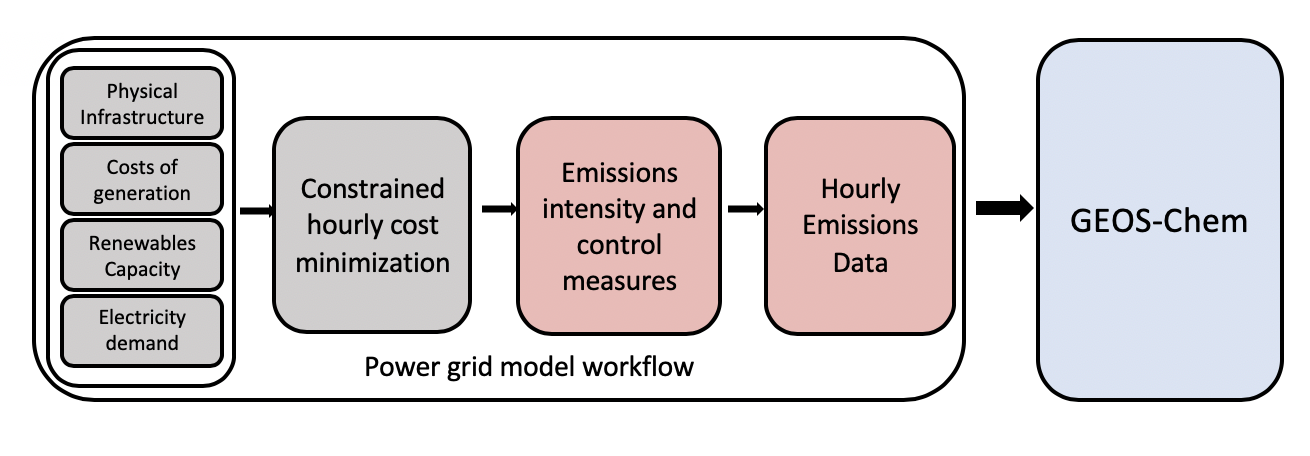
\includegraphics[scale = .5]{US_EGO_flow.png}
    \caption{US-EGO model workflow.}
    \label{fig:model_flow}
\end{figure}

\subsection{US Energy Grid Optimization Model (US-EGO).}
US-EGO is a generator-level cost optimization tool\footnote{This tool was initially developed by Alan Jenn at U.C. Davis for national level assessments that we further modify and validate for state and local assessments. \citep{jenn_future_2018}}. This tool takes all energy generating units (EGU's) across the United States, their capacity, emission factors (for \ce{CO2}, \ce{SO2}, and \ce{NOx}), and their costs for the year 2016, all of which are based on the EPA's National Electric Energy Data System (NEEDS) model v.5.16 \citep{epa_power_2016}. Separating the nation into NEEDS' 64 regions, we use 2016 transmission data (from the NEEDS data) to allow for transmission between each region, and 2016 loads to simulate demand within each region. As the U.S. energy market functions on a Security Constrained Unit Commitment or Security Constrained Economic Dispatch (SCUC/SCED) optimization model, it is fitting to mimic such an optimization in order to model the market \citep{ela_evolution_2014}. The model then optimizes the use of EGUs such that the load matches local generation plus net transmission into the region, at every hour and in every region. The optimization runs across $T$ time periods with 1) $x^{gen}_{i}$ generation for generator $i$ at cost $c^{gen}_{i}$ with $N$ total generators, and 2) $x^{trans}$ transmission power between regions $d$ and $o$ at cost $c_{o\rightarrow{}d}$. This is run for 8760 hours throughout the year, optimizing at each timestep \citep{jenn_future_2018}.
\begin{equation}
    \min\limits_{x^{gen}, x^{trans}}\sum_{i=1}^{N}\sum_{t=1}^{T} x^{gen}_{i}(t) c^{gen}_{i}(t) + \sum_{o,d}\sum_{t=1}^{T} x^{trans}_{o\rightarrow{}d}(t) c^{trans}_{o\rightarrow{}d}(t)
\end{equation}

We restrict transmission such that it mimics the U.S. energy grid, with separation between a western, eastern and Texas grid. Generation for renewable sources of energy, such as hydro, solar, and wind are constrained by maximum possible generation profiles (available from the NEEDS data) at high temporal and spatial resolution. 
The model returns hourly output of generation. From this we calculate the hourly emissions of \ce{SO2}, \ce{NOx}, and \ce{CO_2} by:

\begin{equation}
    x^{gen}_{i}EF_i
\end{equation}

Where $EF_i$ is the emissions factor specific to that EGU. These hourly emissions are merged onto a 0.5\textdegree~by 0.625\textdegree~grid. Validation of the model can be found in the supplemental material.

In order to generate the no-nuclear scenario, we remove all nuclear power plants from the possible set of EGUs. In this scenario, generation cannot match the U.S. energy demand in the summertime in the ERC-REST region (eastern Texas), and therefore we close the gap by adding generators that have prohibitive costs such that they are only utilized when the optimization cannot close. These generators have zero emissions, and are there to allow for the optimization to close, and thus we assume partial blackouts in ERC-REST  without nuclear power during those time periods. 

\begin{figure}
    \centering
    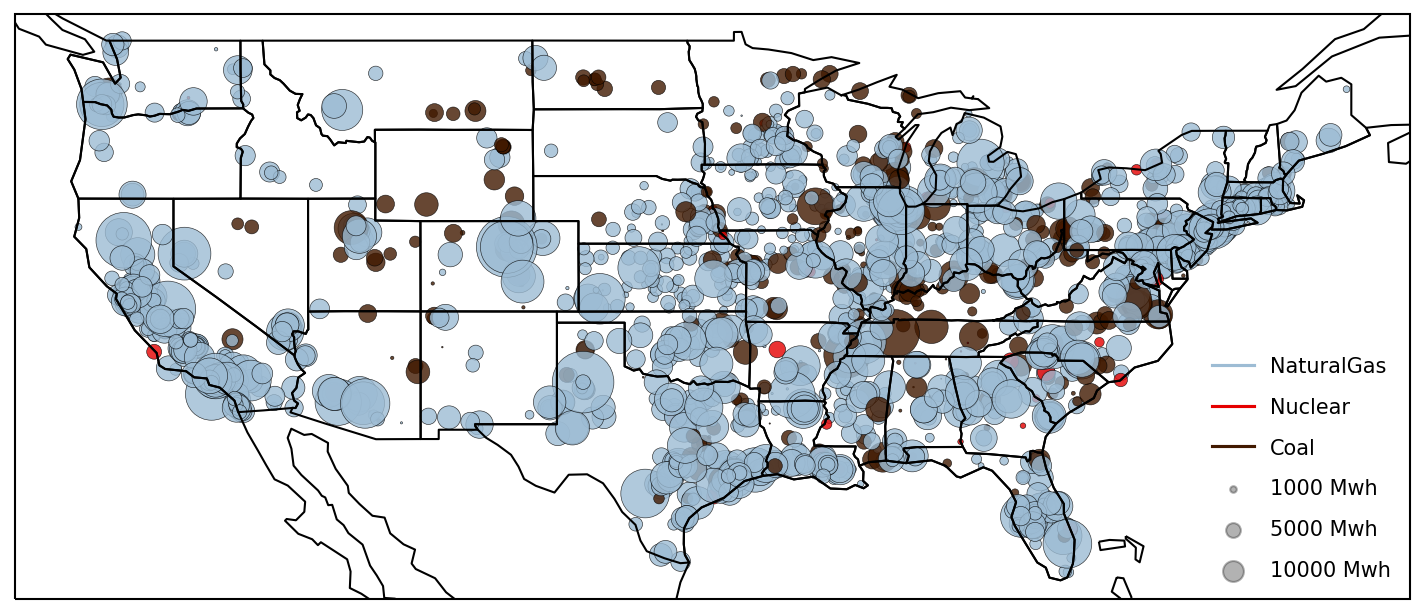
\includegraphics[width=1.\textwidth]{ego_nonuclear_project/Figures/plants_normal.png}
    \caption{Spatial maps of coal, nuclear and natural gas power plants across the U.S. by capacity.} 
    \label{fig:plants}
\end{figure}

\subsection{Chemical Transport Model: GEOS-Chem}
We use the GEOS-Chem model version 13.0.0 \citep{bey_global_2001} to simulate \ce{SO2}, \ce{NOx}, \ce{PM_{2.5}} and ozone concentrations. We use a global horizontal resolution of 4\textdegree x 5\textdegree to create boundary conditions for a nested North American run with horizontal resolution of 0.5\textdegree~by 0.625\textdegree~between 140\textdegree - 40\textdegree W and 10\textdegree - 70\textdegree N. We run full-chemistry in the troposphere only, with 47 vertical levels. Our spin-up is six months, and we analyze daily concentration outputs for the year of 2016. The default EGU emissions for GEOS-Chem are from the 2011 NEI that are scaled to the relevant year \citep{geos-chem_epanei11_2019}, and we also use recently developed emissions inventories for the NEI in 2016. The eGRID simulation utilizes the EPA's Emission and Generation Resource Integrated Database (eGRID) \citep{epa_emissions_2016} \ce{SO2} and \ce{NOx} emissions gridded onto a 0.5\textdegree~by 0.625\textdegree~grid. The US-EGO normal simulation uses the emissions profiles created through the US-EGO model, and the US-EGO no-nuclear scenario uses emissions profiles created through the US-EGO model in a no nuclear scenario. 
\subsection{Monetized Social Cost of Carbon}

\subsection{Health Impact Assessment}

\section{Results and discussion}
\begin{figure}
    \centering
    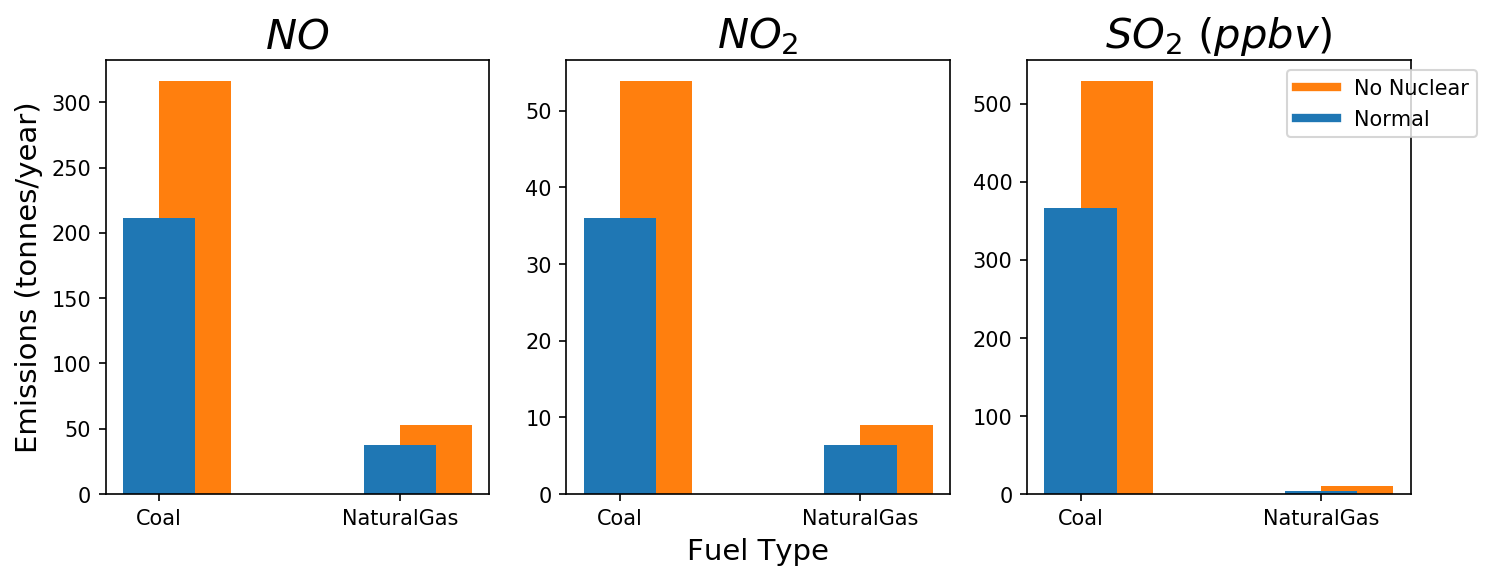
\includegraphics{ego_nonuclear_project/Figures/emissions_fueltype.png}
    \caption{Caption}
    \label{fig:my_label}
\end{figure}
\begin{figure}
    \centering
    \includegraphics{ego_nonuclear_project/Figures/}
    \caption{Caption}
    \label{fig:my_label}
\end{figure}
\begin{figure}
    \centering
    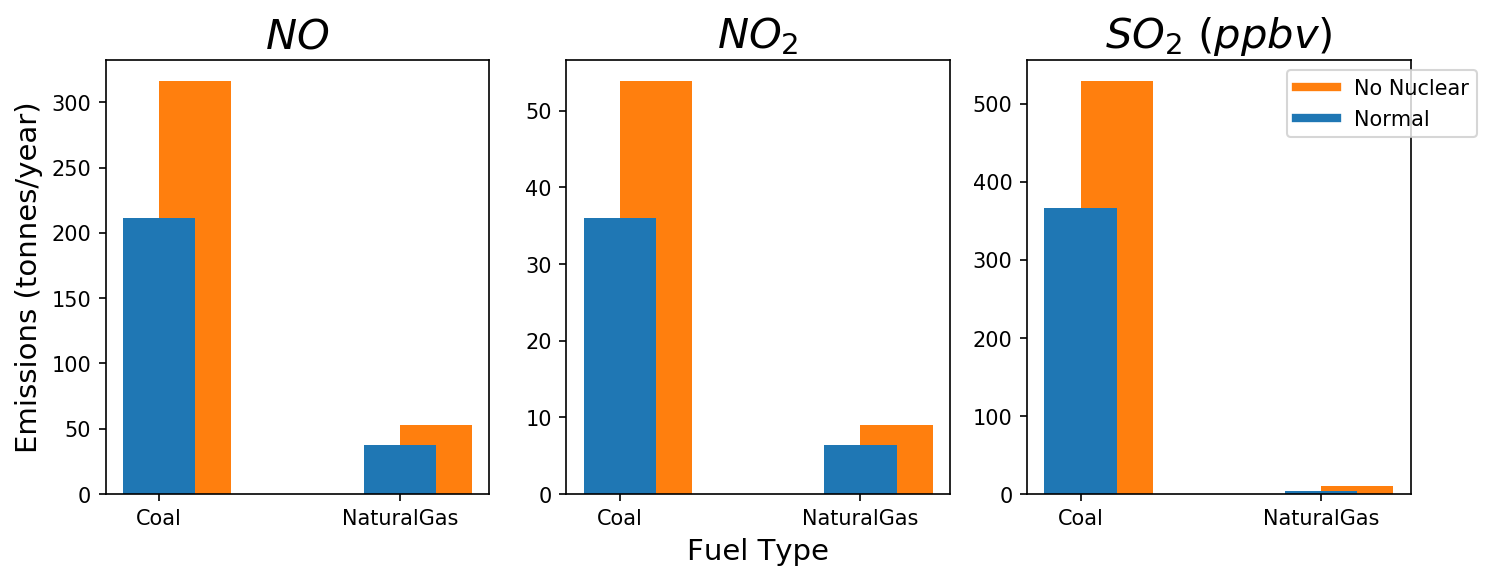
\includegraphics{ego_nonuclear_project/Figures/emissions_fueltype.png}
    \caption{Caption}
    \label{fig:my_label}
\end{figure}
\subsection{References}

The class makes various changes to the way that references are
handled.  The class loads \textsf{natbib}, and also the
appropriate bibliography style.  References can be made using
the normal method; the citation should be placed before any
punctuation, as the class will move it if using a superscript
citation style
\cite{Mena2000,Abernethy2003,Friedman-Hill2003,EuropeanCommission2008}.
The use of \textsf{natbib} allows the use of the various citation
commands of that package: \citeauthor{Abernethy2003} have shown
something, in \citeyear{Cotton1999}, or as given by
Ref.~\citenum{Mena2000}.  Long lists of authors will be
automatically truncated in most article formats, but not in
supplementary information or reviews \cite{Pople2003}. If you
encounter problems with the citation macros, please check that
your copy of \textsf{natbib} is up to date. The demonstration
database file \texttt{achemso-demo.bib} shows how to complete
entries correctly. Notice that ``\latin{et al.}'' is auto-formatted
using the \texttt{\textbackslash latin} command.

Multiple citations to be combined into a list can be given as
a single citation.  This uses the \textsf{mciteplus} package
\cite{Johnson1972,*Arduengo1992,*Eisenstein2005,*Arduengo1994}.
Citations other than the first of the list should be indicated
with a star. If the \textsf{mciteplus} package is not installed,
the standard bibliography tools will still work but starred
references will be ignored. Individual references can be referred
to using \texttt{\textbackslash mciteSubRef}:
``ref.~\mciteSubRef{Eisenstein2005}''.

The class also handles notes to be added to the bibliography.  These
should be given in place in the document \bibnote{This is a note.
The text will be moved the the references section.  The title of the
section will change to ``Notes and References''.}.  As with
citations, the text should be placed before punctuation.  A note is
also generated if a citation has an optional note.  This assumes that
the whole work has already been cited: odd numbering will result if
this is not the case \cite[p.~1]{Cotton1999}.

\subsection{Floats}

New float types are automatically set up by the class file.  The
means graphics are included as follows (Scheme~\ref{sch:example}).  As
illustrated, the float is ``here'' if possible.
\begin{scheme}
  Your scheme graphic would go here: \texttt{.eps} format\\
  for \LaTeX\, or \texttt{.pdf} (or \texttt{.png}) for pdf\LaTeX\\
  \textsc{ChemDraw} files are best saved as \texttt{.eps} files:\\
  these can be scaled without loss of quality, and can be\\
  converted to \texttt{.pdf} files easily using \texttt{eps2pdf}.\\
  %\includegraphics{graphic}
  \caption{An example scheme}
  \label{sch:example}
\end{scheme}

\begin{figure}
  As well as the standard float types \texttt{table}\\
  and \texttt{figure}, the class also recognises\\
  \texttt{scheme}, \texttt{chart} and \texttt{graph}.
  \caption{An example figure}
  \label{fgr:example}
\end{figure}

Charts, figures and schemes do not necessarily have to be labelled or
captioned.  However, tables should always have a title. It is
possible to include a number and label for a graphic without any
title, using an empty argument to the \texttt{\textbackslash caption}
macro.

The use of the different floating environments is not required, but
it is intended to make document preparation easier for authors. In
general, you should place your graphics where they make logical
sense; the production process will move them if needed.

\subsection{Math(s)}

The \textsf{achemso} class does not load any particular additional
support for mathematics.  If packages such as \textsf{amsmath} are
required, they should be loaded in the preamble.  However,
the basic \LaTeX\ math(s) input should work correctly without
this.  Some inline material \( y = mx + c \) or $ 1 + 1 = 2 $
followed by some display. \[ A = \pi r^2 \]

It is possible to label equations in the usual way (Eq.~\ref{eqn:example}).
\begin{equation}
  \frac{\mathrm{d}}{\mathrm{d}x} \, r^2 = 2r \label{eqn:example}
\end{equation}
This can also be used to have equations containing graphical
content. To align the equation number with the middle of the graphic,
rather than the bottom, a minipage may be used.
\begin{equation}
  \begin{minipage}[c]{0.80\linewidth}
    \centering
    As illustrated here, the width of \\
    the minipage needs to allow some  \\
    space for the number to fit in to.
    %\includegraphics{graphic}
  \end{minipage}
  \label{eqn:graphic}
\end{equation}

\section{Experimental}

The usual experimental details should appear here.  This could
include a table, which can be referenced as Table~\ref{tbl:example}.
Notice that the caption is positioned at the top of the table.
\begin{table}
  \caption{An example table}
  \label{tbl:example}
  \begin{tabular}{ll}
    \hline
    Header one  & Header two  \\
    \hline
    Entry one   & Entry two   \\
    Entry three & Entry four  \\
    Entry five  & Entry five  \\
    Entry seven & Entry eight \\
    \hline
  \end{tabular}
\end{table}

Adding notes to tables can be complicated.  Perhaps the easiest
method is to generate these using the basic
\texttt{\textbackslash textsuperscript} and
\texttt{\textbackslash emph} macros, as illustrated (Table~\ref{tbl:notes}).
\begin{table}
  \caption{A table with notes}
  \label{tbl:notes}
  \begin{tabular}{ll}
    \hline
    Header one                            & Header two \\
    \hline
    Entry one\textsuperscript{\emph{a}}   & Entry two  \\
    Entry three\textsuperscript{\emph{b}} & Entry four \\
    \hline
  \end{tabular}

  \textsuperscript{\emph{a}} Some text;
  \textsuperscript{\emph{b}} Some more text.
\end{table}

The example file also loads the optional \textsf{mhchem} package, so
that formulas are easy to input: \texttt{\textbackslash ce\{H2SO4\}}
gives \ce{H2SO4}.  See the use in the bibliography file (when using
titles in the references section).

The use of new commands should be limited to simple things which will
not interfere with the production process.  For example,
\texttt{\textbackslash mycommand} has been defined in this example,
to give italic, mono-spaced text: \mycommand{some text}.

\section{Extra information when writing JACS Communications}

When producing communications for \emph{J.~Am.\ Chem.\ Soc.}, the
class will automatically lay the text out in the style of the
journal. This gives a guide to the length of text that can be
accommodated in such a publication. There are some points to bear in
mind when preparing a JACS Communication in this way.  The layout
produced here is a \emph{model} for the published result, and the
outcome should be taken as a \emph{guide} to the final length. The
spacing and sizing of graphical content is an area where there is
some flexibility in the process.  You should not worry about the
space before and after graphics, which is set to give a guide to the
published size. This is very dependant on the final published layout.

You should be able to use the same source to produce a JACS
Communication and a normal article.  For example, this demonstration
file will work with both \texttt{type=article} and
\texttt{type=communication}. Sections and any abstract are
automatically ignored, although you will get warnings to this effect.

%%%%%%%%%%%%%%%%%%%%%%%%%%%%%%%%%%%%%%%%%%%%%%%%%%%%%%%%%%%%%%%%%%%%%
%% The "Acknowledgement" section can be given in all manuscript
%% classes.  This should be given within the "acknowledgement"
%% environment, which will make the correct section or running title.
%%%%%%%%%%%%%%%%%%%%%%%%%%%%%%%%%%%%%%%%%%%%%%%%%%%%%%%%%%%%%%%%%%%%%
\begin{acknowledgement}

Please use ``The authors thank \ldots'' rather than ``The
authors would like to thank \ldots''.

The author thanks Mats Dahlgren for version one of \textsf{achemso},
and Donald Arseneau for the code taken from \textsf{cite} to move
citations after punctuation. Many users have provided feedback on the
class, which is reflected in all of the different demonstrations
shown in this document.

\end{acknowledgement}

%%%%%%%%%%%%%%%%%%%%%%%%%%%%%%%%%%%%%%%%%%%%%%%%%%%%%%%%%%%%%%%%%%%%%
%% The same is true for Supporting Information, which should use the
%% suppinfo environment.
%%%%%%%%%%%%%%%%%%%%%%%%%%%%%%%%%%%%%%%%%%%%%%%%%%%%%%%%%%%%%%%%%%%%%
\begin{suppinfo}

This will usually read something like: ``Experimental procedures and
characterization data for all new compounds. The class will
automatically add a sentence pointing to the information on-line:

\end{suppinfo}

%%%%%%%%%%%%%%%%%%%%%%%%%%%%%%%%%%%%%%%%%%%%%%%%%%%%%%%%%%%%%%%%%%%%%
%% The appropriate \bibliography command should be placed here.
%% Notice that the class file automatically sets \bibliographystyle
%% and also names the section correctly.
%%%%%%%%%%%%%%%%%%%%%%%%%%%%%%%%%%%%%%%%%%%%%%%%%%%%%%%%%%%%%%%%%%%%%
\bibliography{references}

\end{document}